\documentclass[a4paper]{scrartcl}

%% Language and font encodings
\usepackage[english]{babel}
\usepackage[utf8x]{inputenc}
\usepackage[T1]{fontenc}

%% Sets page size and margins
\usepackage[a4paper,top=2cm,bottom=3cm,left=3cm,right=2cm,marginparwidth=1.75cm]{geometry}

%% Useful packages
\usepackage{amsmath}
\usepackage{graphicx}
\usepackage{subcaption}
\usepackage[colorinlistoftodos]{todonotes}
\usepackage[colorlinks=true, allcolors=blue]{hyperref}
\usepackage{placeins}
\usepackage{siunitx}
\usepackage{sidecap}
\usepackage{float}
\usepackage[format=plain]{caption}
\DeclareSIUnit\atmosphere{atm}

\title{Computational Motor Control - Lab 4}
\author{Florian Kaufmann \and Octave Martin \and Matthias Tsai}

\begin{document}
\maketitle

\section{Modelling the lamprey CPG with phase oscillators}
\subsection{Parameter values for the model (6a.)}

We studied how lamprey CPGs could be modeled with a chain of phase oscillators and first started to explore this model by implementing and simulating different kinds chains of phase oscillators with various parameters. The parameters varied were the number of oscillators, the gradient of frequencies between them and the coupling strength between oscillators. To start off, we chose 10 oscillators, a frequency gradient of $\pi /6$ and a coupling strength of 7 to get an example of a phase-locked chain of oscillators (see Figure \ref{fig:f6a-standard}). From the plots, one can observe that the phase differences between the oscillators all stabilize to constant values and the oscillators visibly synchronize (left plot) by all adopting the same frequency despite of the intrinsic frequency gradient(right plot).

\begin{figure}[!b]
	\centering
	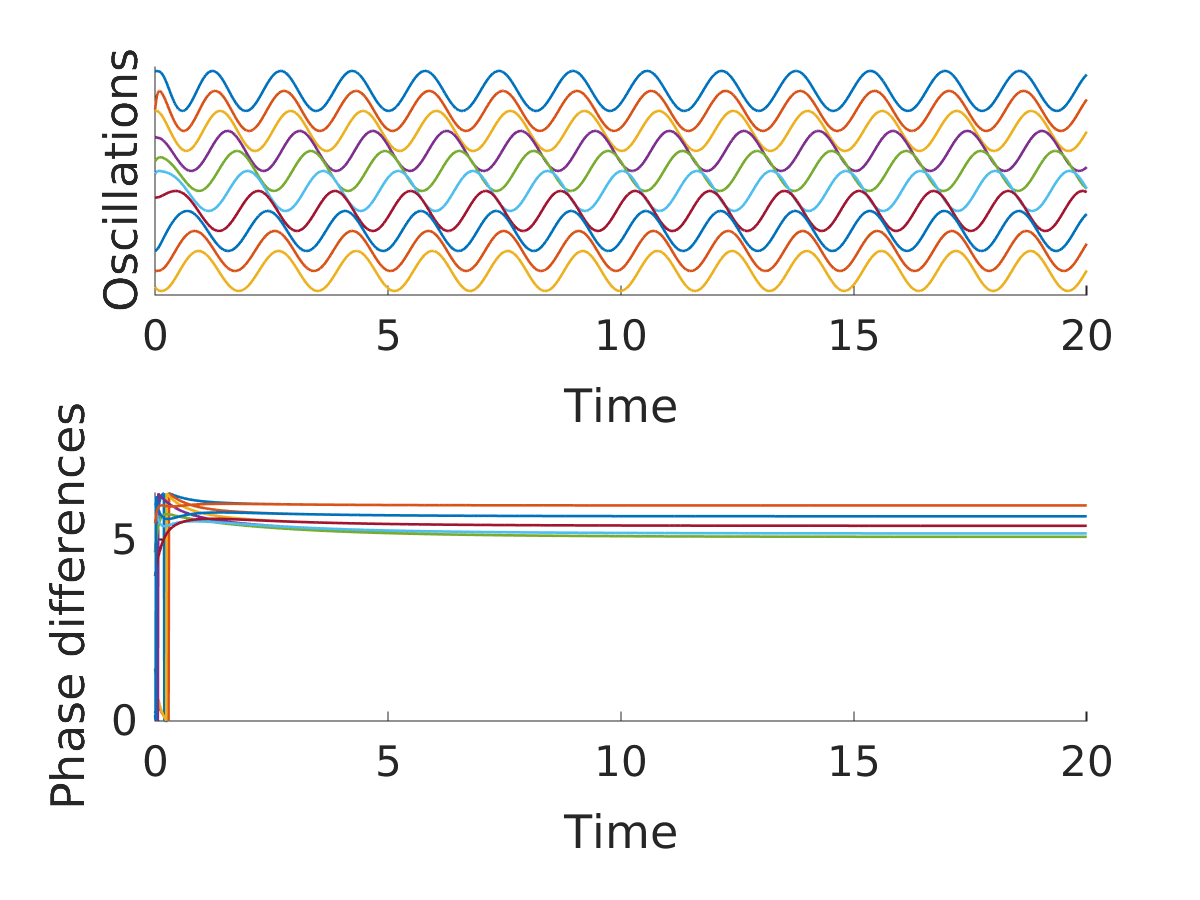
\includegraphics[width=0.5\textwidth]{fig/chain_phase_oscil-6a_stable.png}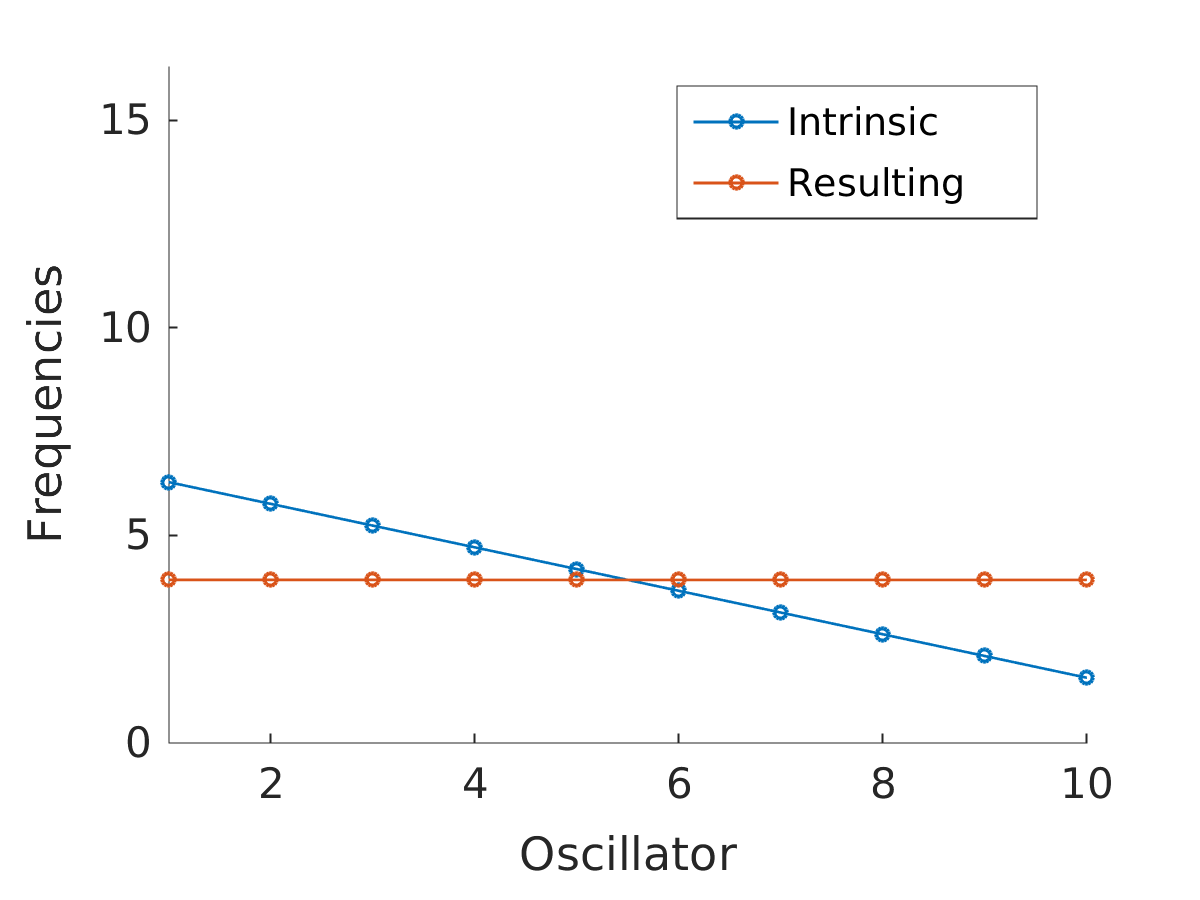
\includegraphics[width=0.5\textwidth]{fig/chain_phase_oscil_freq-6a_stable.png}
	\caption{Simulation of a chain of 10 phase oscillators with frequency gradient of $\pi /6$ and coupling strength of 7. Left: Simulated oscillations and phase differences of the oscillators over time.  Right: Plot of intrinsic frequencies and resulting frequencies from the simulation.}
	\label{fig:f6a-standard}
\end{figure}

Next, we used our analytical formula to sufficiently modify the value of one parameter at a time in order to lose the phase-locked behaviour of the chain of oscillators. First, the coupling strength was modified and reduced to 4 (see Figure \ref{fig:f6a-unstablecoupling}), and as predicted by our analytical model, the phase locking was lost. Interestingly, the chain of oscillators seems to have converged on two distinct frequencies, with the upper half of the chain synchronizing on a higher frequency as the lower part of the chain, with the central oscillators (especially the green one) experiencing an increased instability by being localized at the interface between these two subsystems.

\begin{figure}[!t]
	\centering
	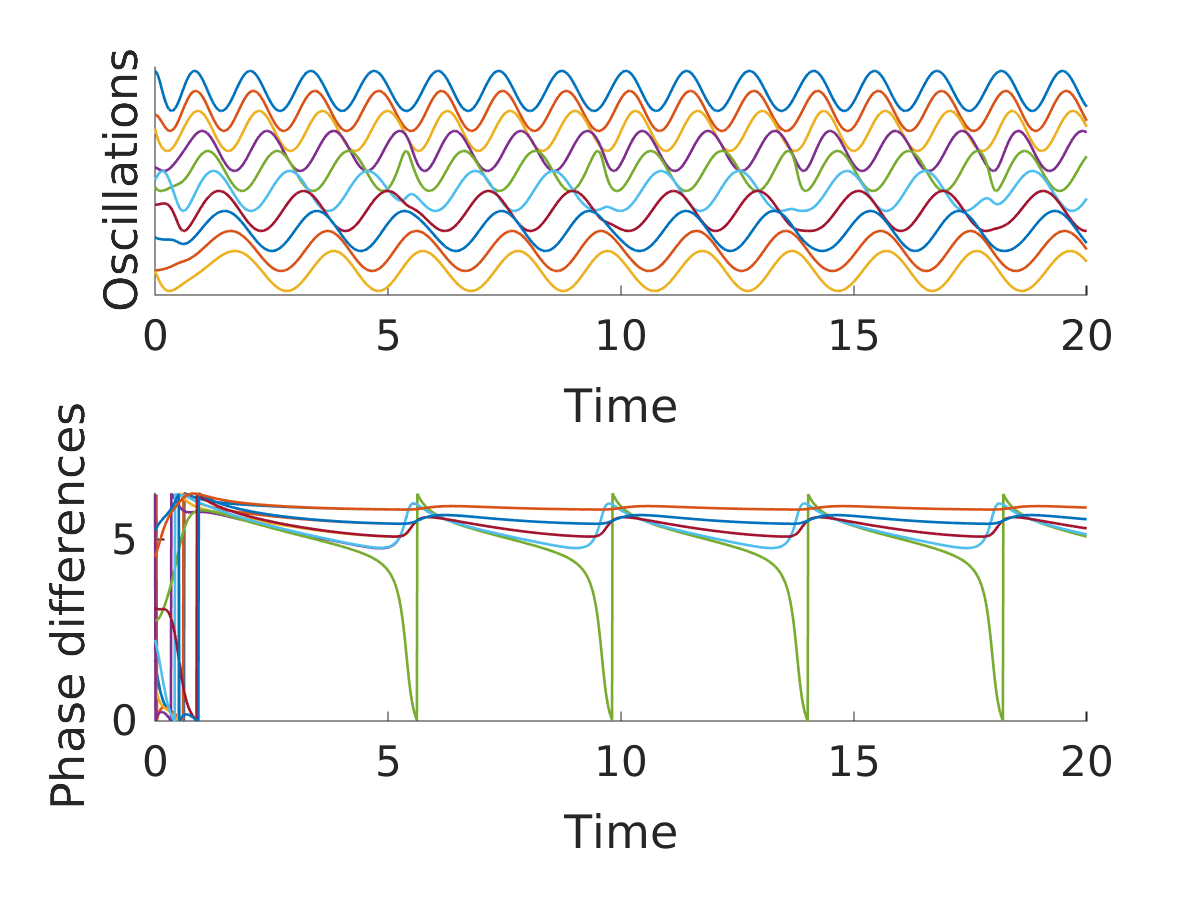
\includegraphics[width=0.5\textwidth]{fig/chain_phase_oscil-6a_unstable.png}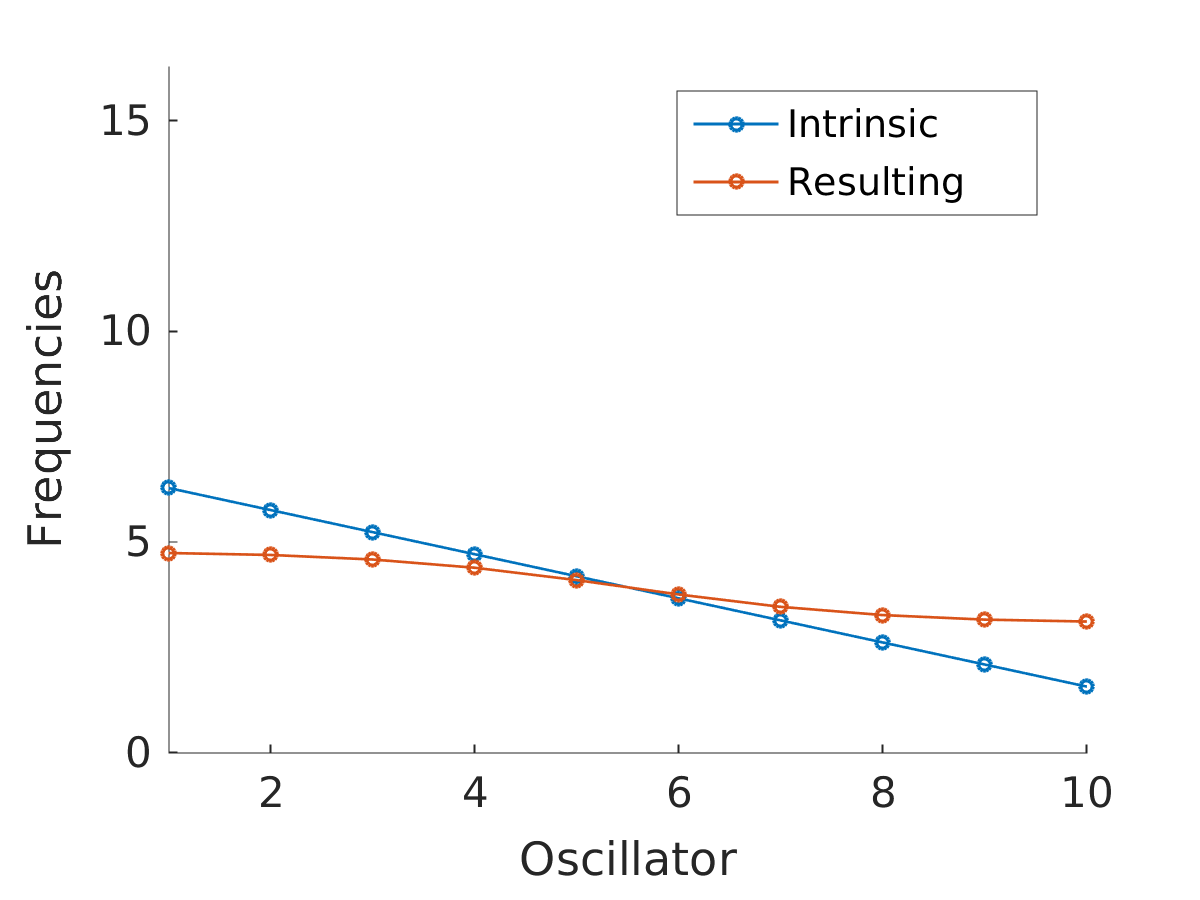
\includegraphics[width=0.5\textwidth]{fig/chain_phase_oscil_freq-6a_unstable.png}
	\caption{Simulation of a chain of 10 phase oscillators with frequency gradient of $\pi /6$ and coupling strength of 4. Left: Simulated oscillations and phase differences of the oscillators over time. Right: Plot of intrinsic frequencies and resulting frequencies from the simulation.}
	\label{fig:f6a-unstablecoupling}
\end{figure}

Similar loss of phase locking was also observed, if our initial phase locked oscillator chain was modified to either raise the frequency gradient to $\pi /5$ or to raise the number of oscillators to 11. This isn't very surprising, because by looking at the phase locking inequality condition using the parameters of our synchronized oscillator chain, one can predict that already a small change of one parameter in the wrong direction would change the sign of the inequality. This is because our chosen standard parameters are already very close to the threshold at which the system loses its phase locking dynamic.

\begin{equation}
	coupling \_ strength = 7 > 6.545 =\frac{\pi \cdot 10^{2}}{6 \cdot 8} = \frac{frequency \_ gradient \cdot Noscils^2}{8}
\end{equation}

In order to get a better idea about how the parameters influence the phase locking, we compared if and how phase differences between oscillators stabilized during the simulations. The standard deviation measures the spread of the variables, therefore the standard deviation of the phase differences between oscillators is constant, if they are synchronized. The standard deviation of the phase differences between oscillators was therefore plotted throughout the simulations using different values for the investigated parameters (see Figure \ref{fig:f6a-phaseSTD}). The first four figures represent such standard deviations of the phase differences between oscillators as a function of time for different values of the system parameters. The simulations were performed for models with linear frequency gradients along the spinal cord and for identical initial conditions. The left column corresponds to models with 10 oscillators and the central column corresponds to models with 20 oscillators. Along the upper row the coupling strength was varied between 1 and 5. Along the lower row the intrinsic frequency gradient was varied between -0.2\,rad/step to -0.001\,rad/step. 

The fifth figure shows Arnold tongues representing the necessary values for coupling strength and frequency gradient for phase locking. The phase locking is verified for couples in the region above the straight lines. The limit condition for a model with 10 oscillators is represented with a dashed line and the limit condition for a model with 20 oscillators is represented with a plain line. Each couple of parameters tested is also plotted, with circles for the variation of the coupling strength (first row) and stars for the variation of the frequency drift (second row).

As expected the simulations and the analytical predictions depicted by the Arnold tongues for phase locking are coherent. For the models with 10 oscillators the simulation for three of the parameter couples present phase locking while only two are phase-locked for the 20 oscillator models. The parameter couple that is phase-locked for 10 oscillators but not for 20 has a coupling strength of 2 and a frequency gradient of -0.2\,rad/step. It is plotted in orange in the four left plots and corresponds to the point in the center of the five points plotted in the Arnold tongue figure.


\begin{figure}[!t]
	\hspace{0.4 cm}\textbf{Chains of 10 oscillators}\hspace{0.9 cm}\textbf{Chains of 20 oscillators}
	
	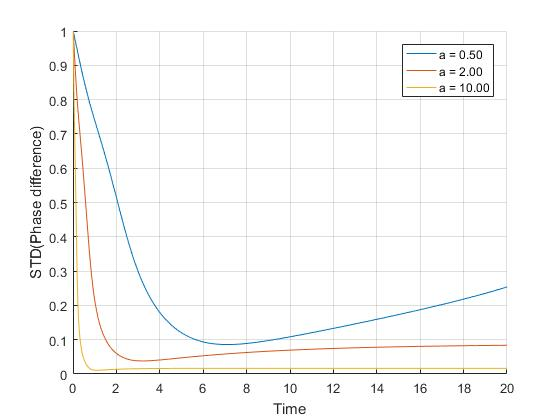
\includegraphics[width=0.33\textwidth]{results/6.a/N10_E_const.jpg}
	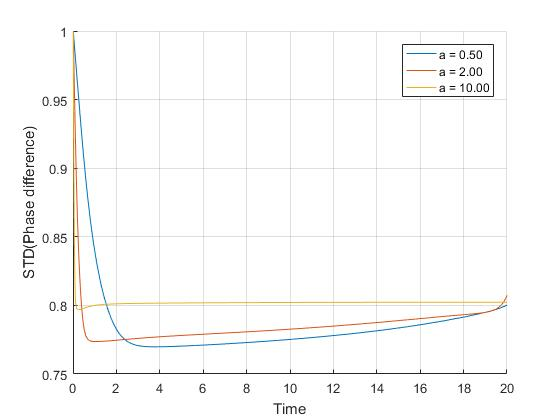
\includegraphics[width=0.33\textwidth]{results/6.a/N20_E_const.jpg}
	
	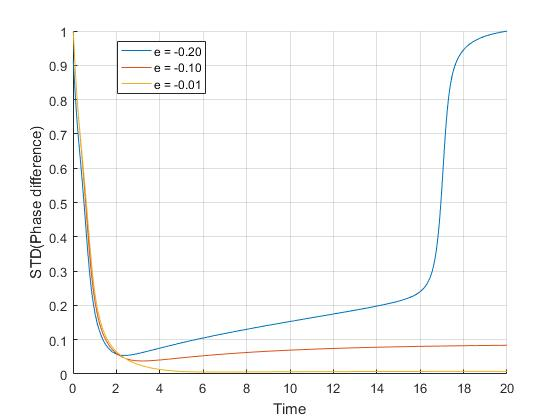
\includegraphics[width=0.33\textwidth]{results/6.a/N10_A_const.jpg}
	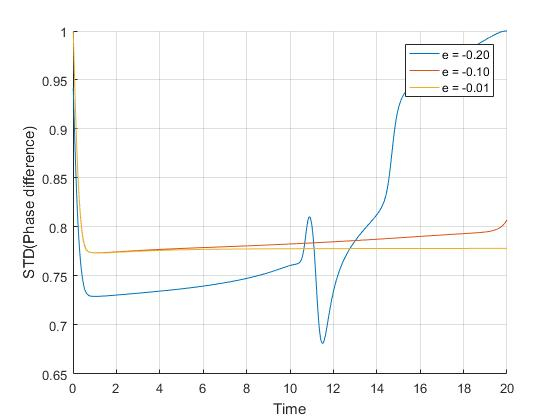
\includegraphics[width=0.33\textwidth]{results/6.a/N20_A_const.jpg}
	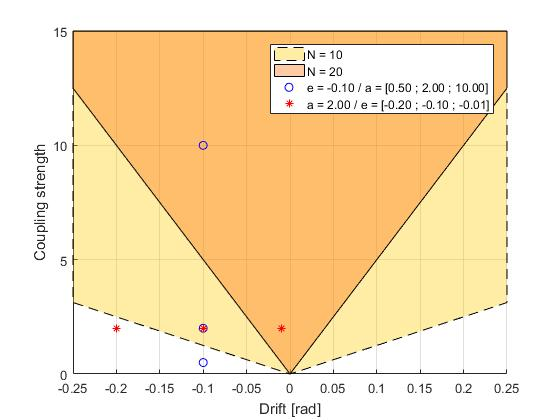
\includegraphics[width=0.33\textwidth]{results/6.a/ArnoldTongue.jpg}
	\caption{Comparison of the standard deviations of the phase gradients between oscillators throughout 20 seconds simulations with different values for the parameters of the CPG model. The two left plots use simulations using chains of 10 oscillators and the two central plots use simulations using chains of 20 oscillators. The upper left and upper central plots use simulations with different values for the coupling strength between oscillators. The lower left and lower central plots use simulations with different values for the linear intrinsic frequency gradient between oscillators. The plot on the right depicts the Arnold tongues corresponding to the parameter subspaces for which phase locking is achieved for chains of either 10 or 20 oscillators. The parameters defining the Arnold tongues are the intrinsic frequency gradients and the coupling strengths between oscillators. Some points are also depicted in the Arnold tongue figure that correspond to the parameter values that were simulated in the four other plots.}
	\label{fig:f6a-phaseSTD}
\end{figure}


\subsection{Non-linear intrinsic frequency gradient (6.b)}

Previous simulations have shown that a linear intrinsic frequency gradient leads to a quadratic phase difference between adjacent oscillators once a stable state has been reached and a sigmoid-like phase difference with respect to the first oscillator of the chain (see Figure \ref{prop}). The stable phase difference with oscillator 1 was found using the cumulative sum of the phase differences between adjacent oscillators. The phase difference between the first and last oscillators is approximatively $2\pi$ i.e. they are in phase as sinus function is $2\pi$-periodic. This correspond to a travelling wave with wavelength equal to the length of the lamprey spinal cord.

In order to study how a different type of intrinsic frequency distribution would influence the model, a simulation was run using a polynomial function to define the intrinsic frequencies of the oscillators (see Figure \ref{stand}). This lead to a sinusoid-like stable phase difference between adjacent oscillators. The stable phase difference with oscillator 1 was found using the cumulative sum of the phase differences between adjacent oscillators. Including the first and last oscillator there are 5 locations where the phase difference with oscillator 1 is null. These points are in phase with each other. This correspond to a standing wave along the lamprey with 5 nodes and therefore 4 anti-nodes.

This is an interesting result, but it is known from biology that the lamprey has constant phase difference between adjacent oscillators while swimming, leading to a linear phase difference to the first oscillator. The linear intrinsic frequency gradient produces a non constant stable phase difference between  adjacent oscillators, which can be seen in figures \ref{3d} and \ref{3e}. It was therefore attempted to reproduce that behaviour with a custom intrinsic frequency distribution (see Figure \ref{3a}). This linear gradient produced a constant phase difference between adjacent oscillators and a linear phase difference with respect to the first oscillator (see Figure \ref{3b}). The simulation that stabilized to a straight wave front is shown in figure \ref{3e}.

\vspace{1cm}

\begin{figure}[h]
	\centering
	\begin{subfigure}[b]{0.49\textwidth}
		\centering
		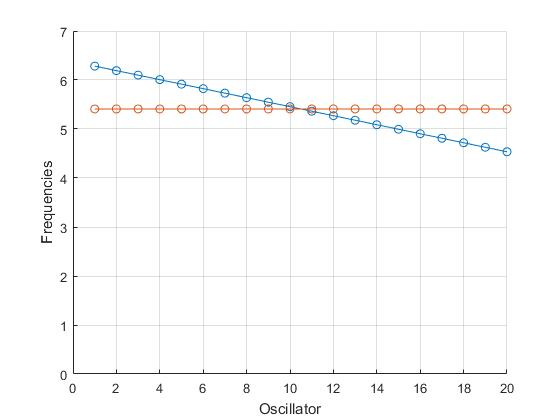
\includegraphics[width=\textwidth]{results/6.b/propaWaveFreq.jpg}
		\caption{}
	\end{subfigure}
	\centering
	\begin{subfigure}[b]{0.49\textwidth}
		\centering
		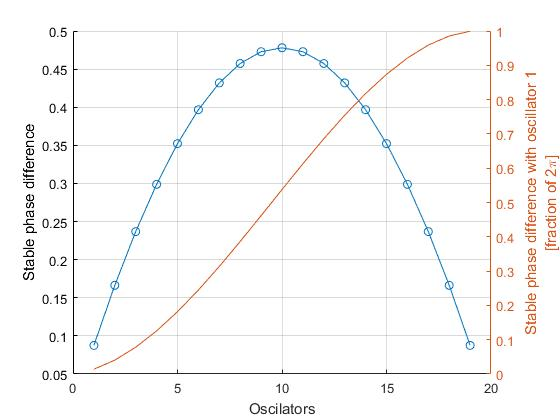
\includegraphics[width=\textwidth]{results/6.b/propaWavePhase.jpg}
		\caption{}
	\end{subfigure}
	\caption{Intrinsic and resulting frequencies for each oscillator (a). Stable phase difference between adjacent oscillator and with first oscillator (b). The simulation was performed with 20 oscillators, a coupling strength of 10 and a linear gradient of intrinsic frequencies with drift -0.092\,rad/step. These simulation parameters fulfill the phase locking condition.}\label{prop}
\end{figure}

\vspace{1cm}

\begin{figure}[!b]
	\centering
	\begin{subfigure}[b]{0.49\textwidth}
		\centering
		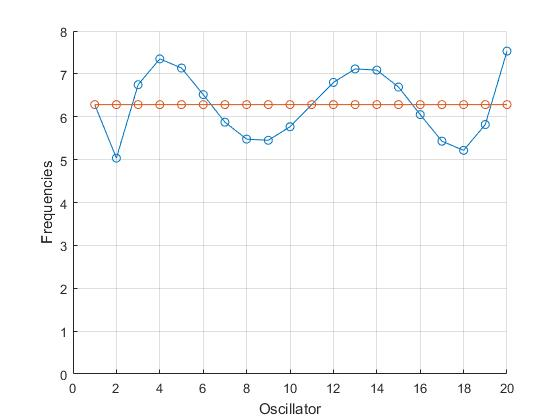
\includegraphics[width=\textwidth]{results/6.b/standWaveFreq.jpg}
		\caption{}
	\end{subfigure}
	\centering
	\begin{subfigure}[b]{0.49\textwidth}
		\centering
		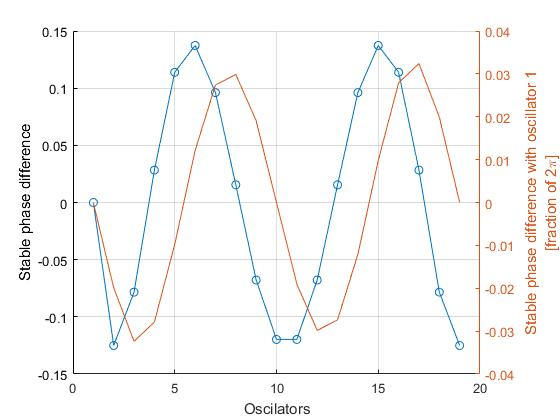
\includegraphics[width=\textwidth]{results/6.b/standWavePhase.jpg}
		\caption{}
	\end{subfigure}
	\caption{Intrinsic and resulting frequencies for each oscillator (a). Stable phase difference between adjacent oscillator and with first oscillator (b). The simulation was performed with 20 oscillators, a coupling strength of 10 and a polynomial gradient of intrinsic frequencies: $\omega_i = \omega_{1} + (-1.95\ 10^{-6}\times(i-1)^7 -1.37\ 10^{-4}\times(i-1)^6) -3.56\ 10^{-6}\times(i-1)^5 +4.12\ 10^{-2}\times(i-1)^4 -1.76\ 10^{-1}\times(i-1)^3 -2.43\ 10^{-1}\times(i-1)^2 +3.16\times(i-1)-4.02$. The simulation parameters fulfill the phase locking condition (i.e. the absolute value of the components of vector S are all inferior or equal to 1).}\label{stand}
\end{figure}

\begin{figure}[!b]
	\centering
	\begin{subfigure}[b]{0.49\textwidth}
		\centering
		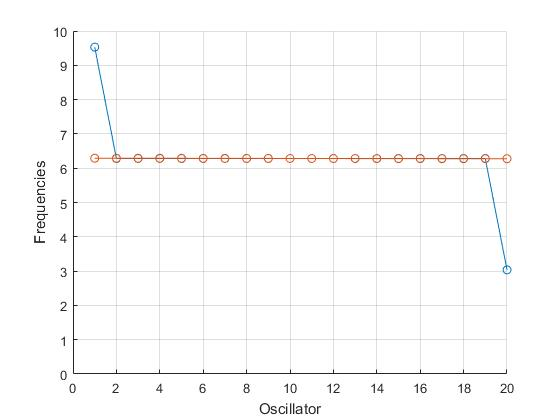
\includegraphics[width=\textwidth]{results/6.b/compSP_DP_CPFreq.jpg}
		\caption{}\label{3a}
	\end{subfigure}
	\centering
	\begin{subfigure}[b]{0.49\textwidth}
		\centering
		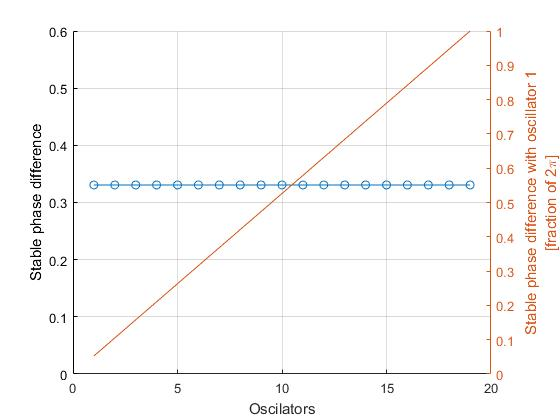
\includegraphics[width=\textwidth]{results/6.b/compSP_DP_CPPhase.jpg}
		\caption{}\label{3b}
	\end{subfigure}
	\centering
	\begin{subfigure}[b]{0.49\textwidth}
		\centering
		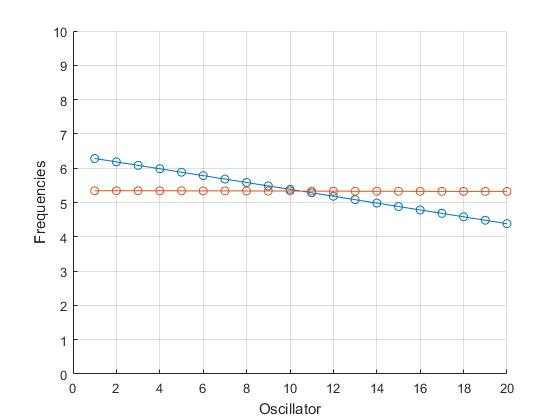
\includegraphics[width=\textwidth]{results/6.b/compSP_DP_DPFreq.jpg}
		\caption{}\label{3c}
	\end{subfigure}
	\centering
	\begin{subfigure}[b]{0.49\textwidth}
		\centering
		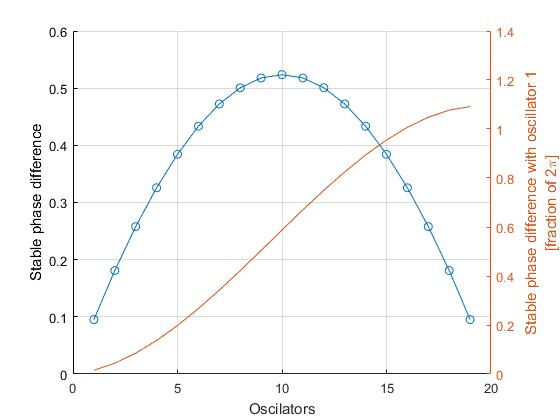
\includegraphics[width=\textwidth]{results/6.b/compSP_DP_DPPhase.jpg}
		\caption{}\label{3d}
	\end{subfigure}
	\begin{subfigure}[b]{\textwidth}
		\centering
		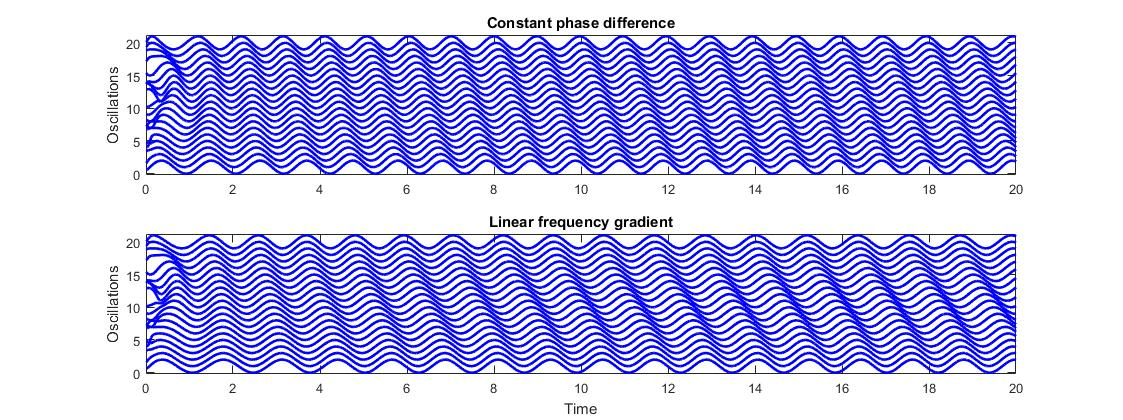
\includegraphics[width=\textwidth]{results/6.b/compSP_DP_oscillations.jpg}
		\caption{}\label{3e}
	\end{subfigure}
	\caption{Intrinsic and resulting frequencies for each oscillator (\ref{3a}, \ref{3c}). Stable phase difference between adjacent oscillator and with first oscillator (\ref{3b}, \ref{3d}). The simulations were performed for non linear gradient (\ref{3a}, \ref{3b}) given by: $\omega_{1} = 2\pi + 3.2469 ,\omega_{20} = 2\pi - 3.2469 , \omega_{i} = 2\pi$ for i = [2,19] and for a linear gradient (\ref{3c}, \ref{3d}) with drift -0.1\,rad/step. For all the simulations the number of oscillators was 20 and the coupling strength 10. The same initial conditions were used for both simulations. Simulated oscillation as a function of time (\ref{3e}) for both intrinsic frequency models.}
\end{figure}


\subsection{External load (6.c)}
In this part an external load with frequency $\omega_{mech}$ is applied to the tail of the lamprey with a sensory coupling strength $a_{sens}$:
\begin{align*}
\frac{d}{dt}\psi_N &= \omega_N + a \sin(\psi_{N-1}-\psi_N) + a_{sens} \sin(\omega_{mech}.t-\psi_N) \\
\frac{d}{dt}\mathbf{\phi} &= \mathbf{\Omega} + A \mathbf{S} - a_{sens} \sin(\omega_{mech}.t-\psi_N)\ [0, \ldots, 0,\, 1]'
\end{align*}

\vspace{0.5cm}

And therefore in phase locking regime:
\begin{align*}
\frac{d}{dt}\mathbf{\phi} &= 0\\
\mathbf{S} &= A^{-1}(a_{sens}\sin(\omega_{mech}.t-\psi_N)\ [0, \ldots, 0,\, 1]'-\mathbf{\Omega})
\end{align*}

\vspace{0.5cm}

The condition for phase locking is that for every element $s_i$ of $\mathbf{S}$: $|s_i|\leq1$.
Therefore setting the coupling strength to 10 and the frequency drift to -0.1\,rad/step, and as $-1\leq\sin(x)\leq1 \forall x \in \mathbf{R}$, we can calculate a value for the sensor coupling strength such that the condition for phase locking is verified.

We studied the effect of the sensor coupling strength and mechanical excitation frequency on the resulting frequency of the oscillators (see Figure \ref{4a} and \ref{4c}) while checking for phase locking conditions using the standard deviation of the phase differences between oscillators as a measure of phase locking (see Figure \ref{4b} and \ref{4d}). As expected, for the chosen set of parameters the standard deviation of the phase differences between the oscillators is bounded with small periodic perturbation corresponding to small variations of the few last oscillators. We can conclude that the system is in a phase locking regime in a less strict sense than in the previous sections.

From figure \ref{4c} one can observe that the effect of sensor coupling affects more strongly the last oscillator and that its resulting frequency converges towards the frequency of mechanical excitation. The frequency of the first oscillator also increases for high sensor coupling strengths.

From the figure \ref{4a} we can see that there is a range of excitation's frequencies ($0.8\times2\pi-0.95\times2\pi$\,rad/s) for which the last oscillator converges to $\omega_{mech}$ and the frequency of the first oscillator increases steadily. This range is close from the resulting frequency of the oscillator without mechanical excitation which is around $0.85\times2$. For higher excitations frequencies the frequency drops possibly because the intrinsic and excitation oscillations compensates each other. Neither the last nor the first oscillator frequencies converges toward $\omega_{mech}$ at higher mechanical excitation frequencies.
It seems that this sensory input can thus modulate the oscillations of the last oscillators of the chain. One can therefore hope to use this property to better tune the phase differences between the oscillators in order to get the linear phase gradient observed in nature and already proved to be reproducible (see figure \ref{4a}). By thus implementing a sensory input with low intrinsic frequency and a coupling strength dependent on the phase difference between the last oscillator and its neighbour, it becomes possible to show that a well tuned sensory input can help the oscillator dynamics to become closer to the dynamics naturally observed in the lamprey (see figure \ref{fig:sensoryphase}). Indeed, with this sensory input the phase gradient becomes more linear than the phase gradient from the simulation without sensory input (the parameters used for the simulations were: 20 oscillators, intrinsic frequency gradient of -0.06\,rad/step and a coupling strength of 10).

\begin{figure}[t]
	\centering
	\begin{subfigure}[b]{0.49\textwidth}
		\centering
		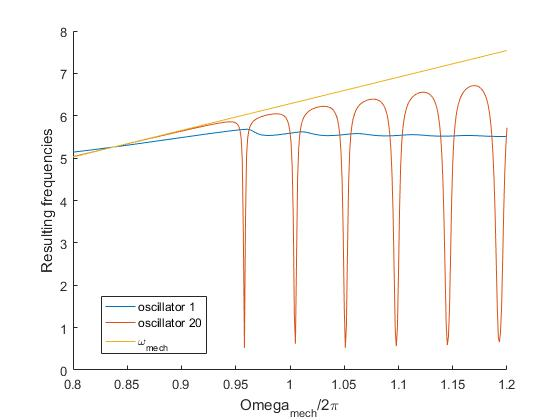
\includegraphics[width=\textwidth]{results/6.c/Freq_A_const.jpg}
		\caption{}\label{4a}
	\end{subfigure}
	\centering
	\begin{subfigure}[b]{0.49\textwidth}
		\centering
		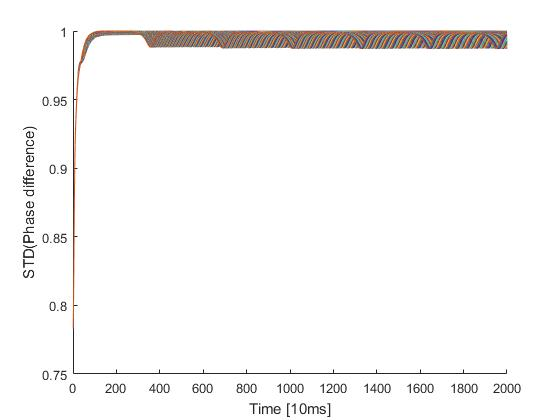
\includegraphics[width=\textwidth]{results/6.c/Phase_A_const.jpg}
		\caption{}\label{4b}
	\end{subfigure}
	\centering
	\begin{subfigure}[b]{0.49\textwidth}
		\centering
		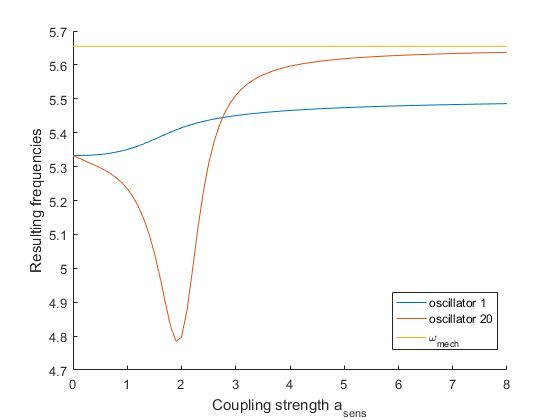
\includegraphics[width=\textwidth]{results/6.c/Freq_O_const.jpg}
		\caption{}\label{4c}
	\end{subfigure}
	\centering
	\begin{subfigure}[b]{0.49\textwidth}
		\centering
		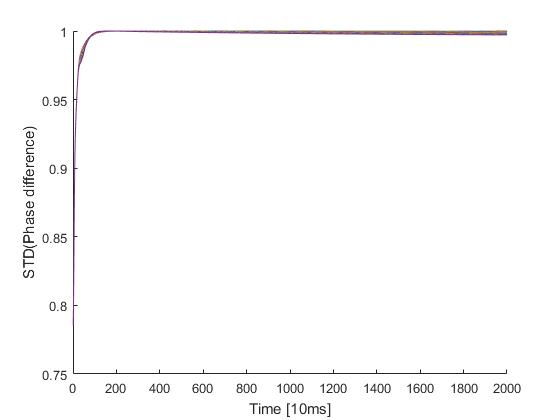
\includegraphics[width=\textwidth]{results/6.c/Phase_O_const.jpg}
		\caption{}\label{4d}
	\end{subfigure}
	\caption{Resulting frequencies of the oscillator 1 and 20 as well as mechanic excitation(\ref{4a}-\ref{4c}). In figure \ref{4a} the coupling strength was kept constant at 8 while the frequency of the mechanic excitation was varied. In figure \ref{4c} the mechanic excitation's frequency was kept constant while the coupling strength was varied. Figures \ref{4b} and \ref{4d} represent the normalized standard deviation of the phase difference between oscillators as a function of time to check for phase locking. All the simulations were done for models with coupling strength of 10, frequency drift of -0.1\,rad/step and 20 oscillators.}
\end{figure}

\begin{figure}[b]
	\centering
	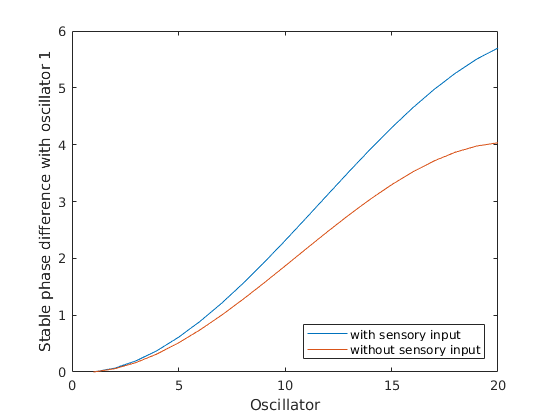
\includegraphics[width= 0.5\textwidth]{fig/figure6c_phasediff-sensory.png}
	\caption{Stable phase differences of the oscillators with or without a sensory input modelled by a smart input to the last oscillator with an intrinsic frequency and a coupling strength.}
	\label{fig:sensoryphase}
\end{figure}

\FloatBarrier

\section{Comparing neuronal oscillators with phase oscillators}
\subsection{General behaviour (7.a)}

We saw in the previous section that coupled phase oscillators could synchronize although they had different intrinsic frequencies and used this as a basis to model CPGs of the lamprey. Phase oscillators are a theoretical model however; it is thus of interest to find out, if the same results can be achieved using a more biological basis. This section was therefore devoted to study how coupled neuronal oscillators could produce the same type of CPGs as phase oscillators. This idea was tested by simulating two couples of neural oscillators with different coupling strengths between the couples (see figure \ref{2phase}). This shows that coupled neural oscillators work in a similar way as coupled phase oscillators in the sense that they will not synchronize to be phase-locked, if their coupling strength is to weak, but can if it is sufficiently strong. 



An obvious difference with the chain of phase oscillators seen in the previous section is that coupled neural oscillators  seem to produce less clean sinusoidal oscillations. Another difference is that, if the coupling strength is set to high, the neural system loses its oscillatory behaviour (see figure \ref{kill}). Such a simulation shows that the "primary" or coupled neurons (neurons 1 and 3) will become very strongly activated and the "secondary" neurons (neurons 2 and 4) will seemingly die. This behaviour seems to arise from the fact that if the primary neurons have a strong symmetric coupling strength between each other, this will lead to a positive feedback loop that leads them to stay strongly activated. Due to this strong activation and the negative weight from the primary neurons to the secondary neurons will be strongly repressed, thus explaining their seemingly premature death. 



\begin{figure}[!b]
	\centering
	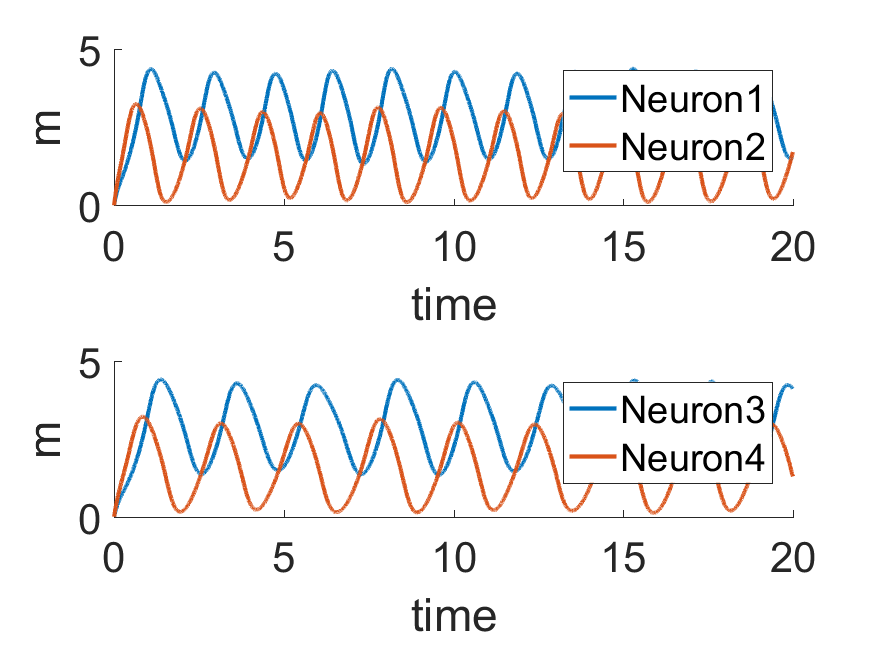
\includegraphics[width=0.5\textwidth]{fig/neuron1.png}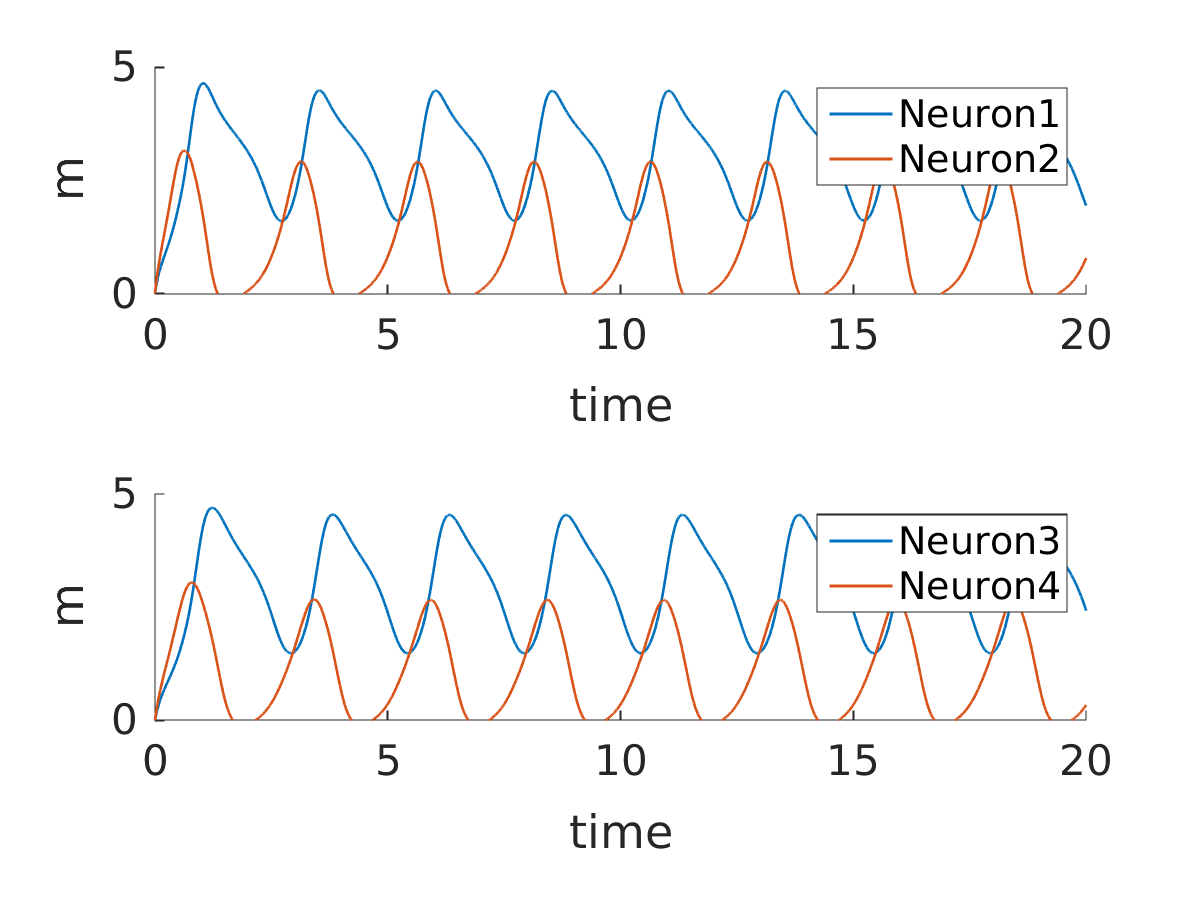
\includegraphics[width=0.5\textwidth]{fig/figure7a_coupledneurons.png}
	\caption{Simulation of two coupled neural oscillators with different intrinsic frequencies. Neurons 1 and 2 have time constants of 0.6 and neurons 3 and 4 have time constants of 0.8. Left: symetric coupling strength of 0.1. Right: symetric coupling strength of 0.3.}\label{2phase}
\end{figure}

This epilepsy-like behaviour of some neurons hyper-activating and killing the activity of other neurons if not very desirable for our model. However, it turns out that there is a way to avoid it. By using negative coupling strengths similar results can be achieved as for positive coupling strengths if the amplitude of the coupling remains small. This means that weak negative coupling will usually not lead to synchronization, but strong coupling strengths between primary neurons will. The important difference is that even for strong coupling with amplitudes that would disrupt the oscillation behaviour for the case of positive coupling, in the case of negative coupling this doesn't happen (see figure \ref{crazy}). Indeed, the periodic behaviour of the neurons is maintained as well as the synchrony. However, the signal form looks less sinusoidal with increasing coupling strength amplitude. This dynamics might not be appropriate, if they were to be directly translated into motion, but since neurons first relay to other neurons or at least to muscle before forces and motion is generated, there is no better reason to believe that one of the wave forms should be better than the other for that purpose. In the opposite, one could conjecture that this variable dynamic might facilitate the generation of more varied patterns of motion by the spinal cord. 

Finally, one should note the maybe too obvious fact that likewise the phase oscillators, if the coupled neural oscillators have a too big difference in intrinsic frequency, they will not be able to synchronize. Overall, this show that this neural model seems to be able to fairly well reproduce the dynamics of two coupled phase oscillators. The more precise dependence is investigated in the last section by approximating the Arnold tongue describing the stability of the system depending on the values of the intrinsic frequency difference and the coupling strength (see Figure \ref{fig:bonus}).

\begin{figure}[!h]
	\centering
	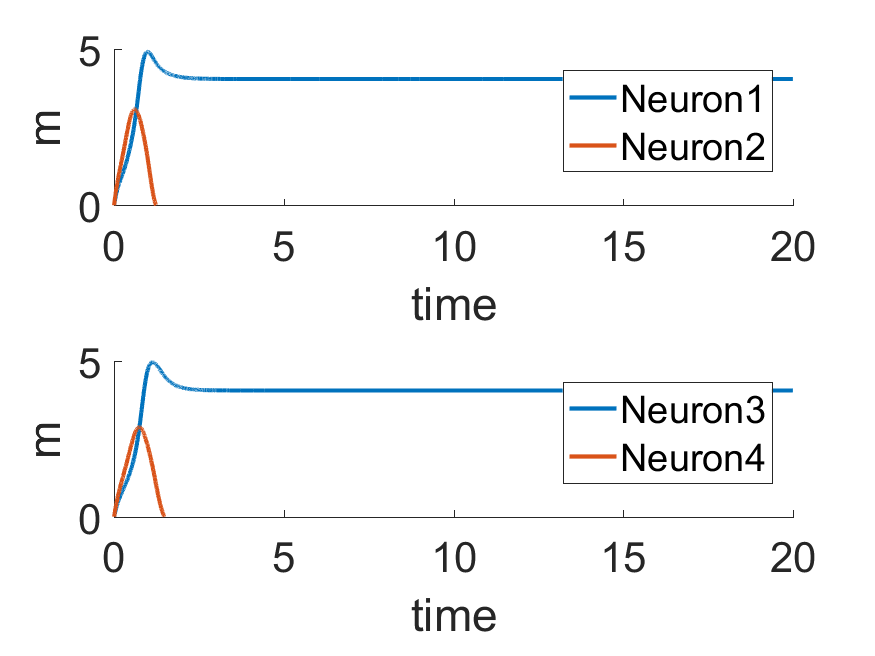
\includegraphics[width=0.5\textwidth]{fig/kill.png}
	\caption{Simulations of coupled neural oscillators with strong symmetric positive coupling strength between neurons 1 and 3}\label{kill}
\end{figure}

\begin{figure}[!h]
	\centering
	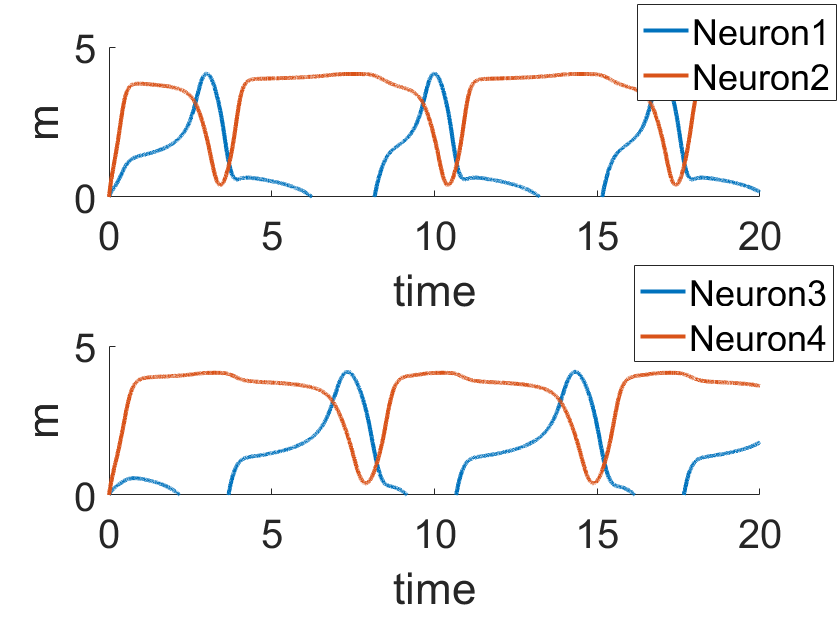
\includegraphics[width=0.5\textwidth]{fig/crazy.png}
	\caption{Simulations of coupled neural oscillators with strong symmetric negative coupling strength between neurons 1 and 3}\label{crazy}
\end{figure}



\newpage
\subsection{Comparing forced oscillators (7.b)}

It is known from biology that CPGs are usually not open-loop, but closed-loop controllers and are modulated by sensory input. Furthermore, upper investigations of the effect of a sensory input on the chain of phase oscillator could improve the model. This is a convincing motivation to also study how sensory inputs could be incorporated in our system of coupled neural oscillators.
A model incorporating a sensory input acting on a primary neuron (neuron 1) was therefore simulated (see Figure \ref{fig:7b-lowfreq}). This showed that, if the coupling to neuron 1 was sufficient and the exerted frequency of the sensory input was reasonably close to the intrinsic frequency of the neural oscillator, the sensory input could force its own frequency upon the neural oscillator, which would also keep synchronized to the second neural oscillator to which it was coupled. This resulted in both neural oscillators synchronizing at the frequency of the sensory input.

\begin{figure}[!b]
	\centering
	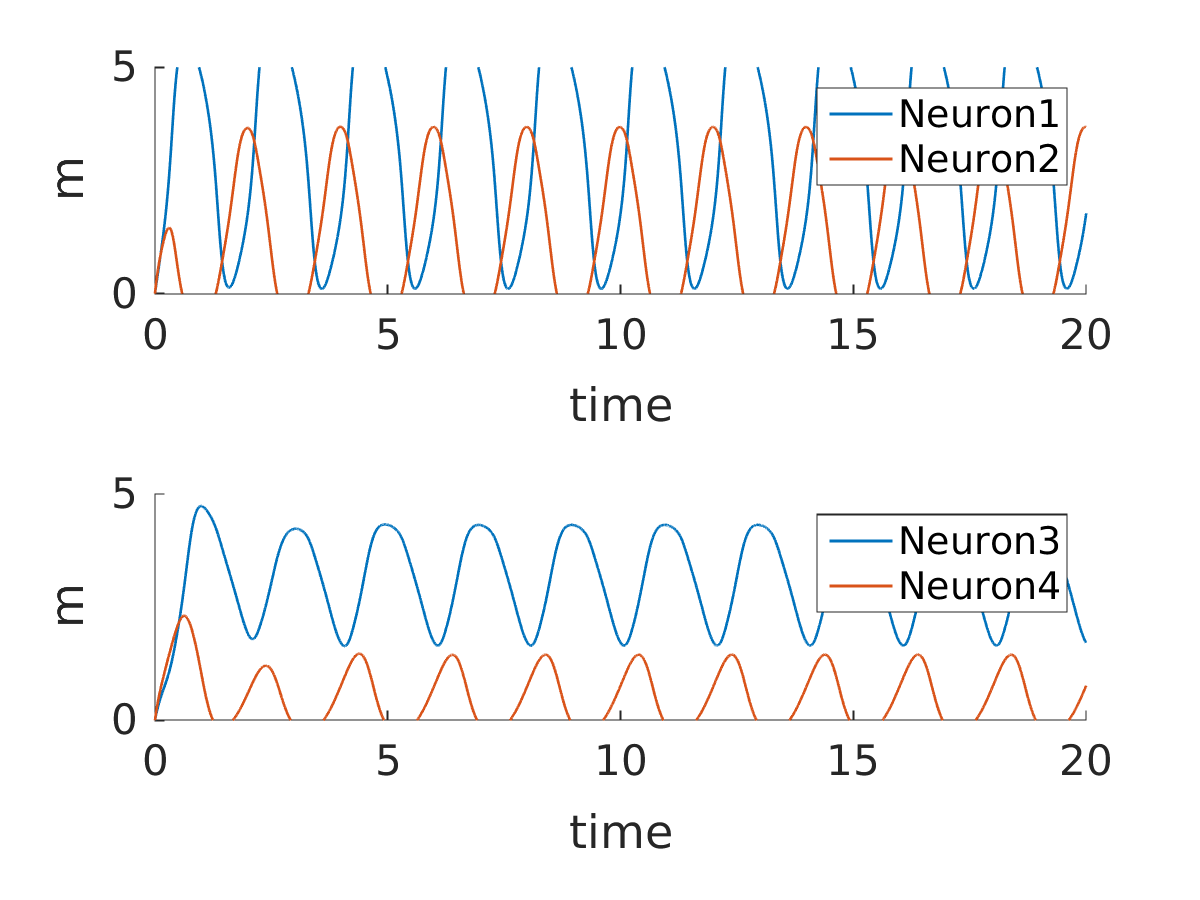
\includegraphics[width=0.5\textwidth]{fig/figure7b_lowfreq-simu.png}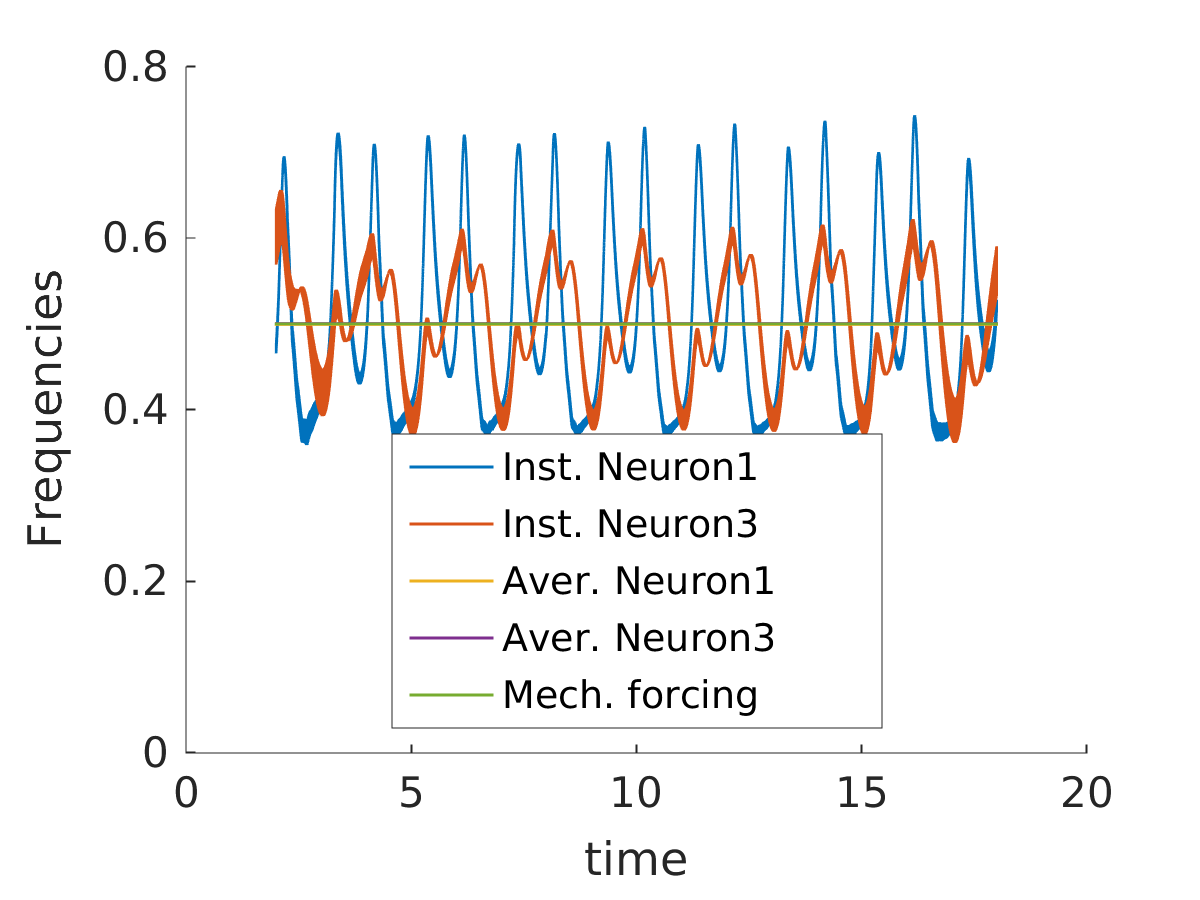
\includegraphics[width=0.5\textwidth]{fig/figure7b_lowfreq-freq.png}
	\caption{Simulation of two coupled neuronal oscillators with time constants 0.06 and 0.08 and with symmetric coupling strengths of 0.5. Neuron 1 is also subject to a sensory input modelled as a coupled oscillator with coupling strength of 1 and frequency of $\pi$. Left: Plot of the simulated neurons in time. Right: Plot of the resulting frequencies of neurons 1 and 3.}
	\label{fig:7b-lowfreq}
\end{figure}

\begin{figure}[!b]
	\centering
	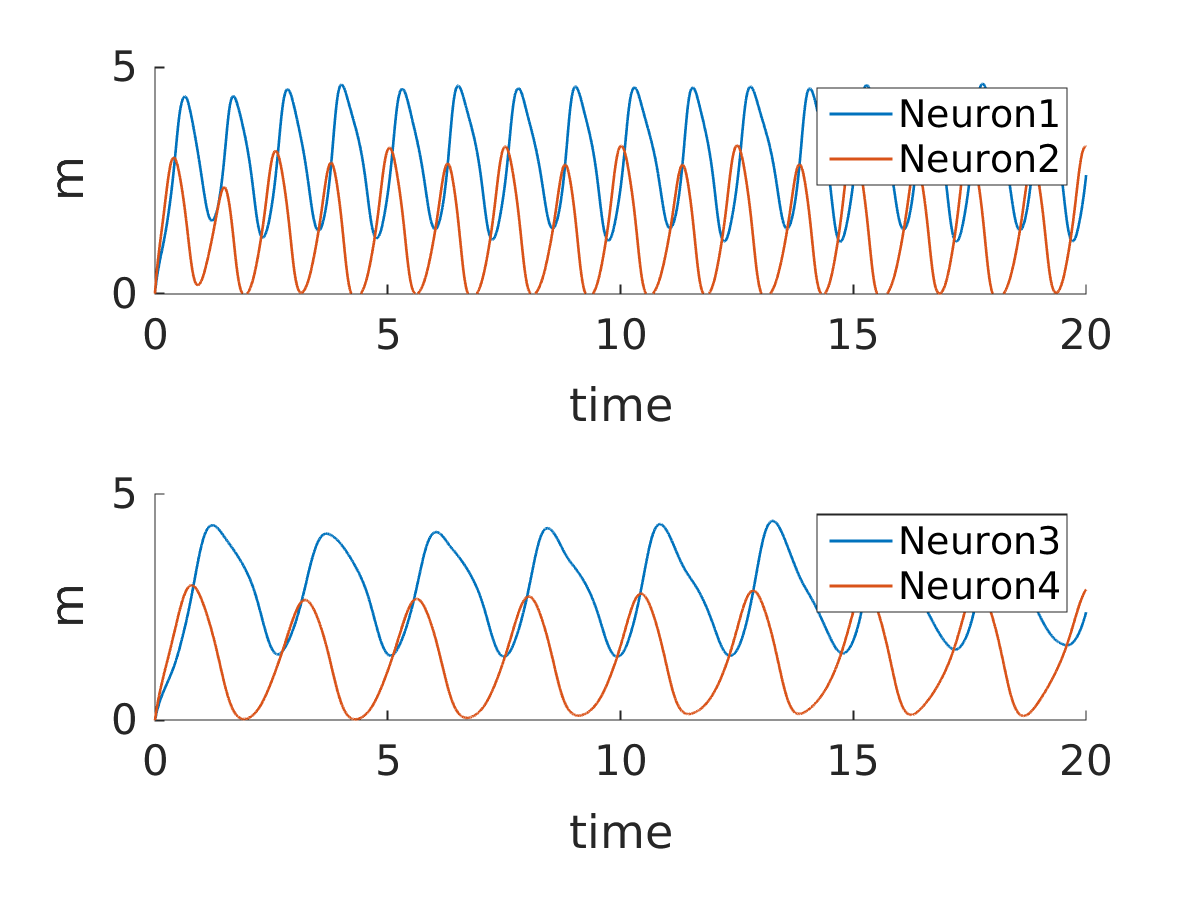
\includegraphics[width=0.5\textwidth]{fig/figure7b_highfreq-simu.png}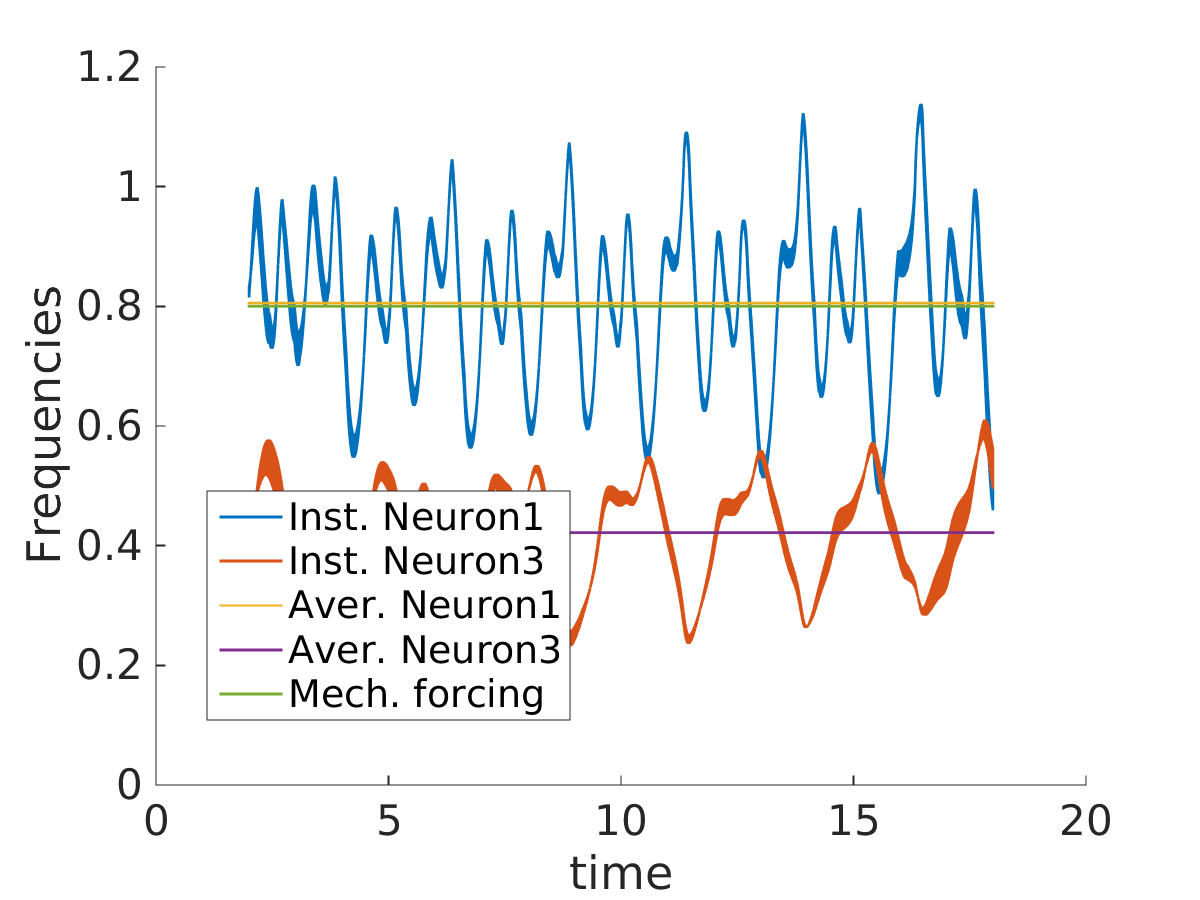
\includegraphics[width=0.5\textwidth]{fig/figure7b_highfreq-freq.png}
	\caption{Simulation of two coupled neuronal oscillators with time constants 0.06 and 0.08 and with symmetric coupling strengths of 0.5. Neuron 1 is also subject to a sensory input modelled as a coupled oscillator with coupling strength of 1 and frequency of $1.6\pi$. Left: Plot of the simulated neurons in time. Right: Plot of the resulting frequencies of neurons 1 and 3.}
	\label{fig:7b-highfreq}
\end{figure}

However, if the frequency of the sensory input is to different of the intrinsic frequencies of the neural oscillators, they will not be able to synchronize at this mechanical frequency. An example of such a system was simulated and is depicted in figure \ref{fig:7b-highfreq}. For this simulation, all parameters are the same as for the simulation of figure \ref{fig:7b-lowfreq} only the frequency of the mechanical input is 1.6 times higher. One can observe that although the second oscillator didn't synchronize to the mechanical frequency, the first oscillator which was directly coupled to the sensory input did. One can thus interpret that the second oscillator didn't synchronize, because the coupling strength between oscillators was to weak and the intrinsic frequency of the second oscillator was to different from the mechanical frequency to be able to align with it.

One can now ask the question about what happens, if the sensory input has a very strong coupling and a very high frequency, but the neural oscillators also have a strong coupling strength. Intuitively one would believe that synchrony should be maintained as long as the coupling strength between the neural oscillators is strong enough. Such a scenario was simulated using a strong positive coupling strength (see Figure \ref{sat}). It shows that the positive coupling will again lead to an over-excitation of the primary neurons and strong repression of the secondary neurons. In this case however, an oscillation can be maintained thanks to the sensory input which is transmitted to the second oscillator through the strong coupling between the two neural oscillators. One might therefore hypothesise that a sensory input might help to jump start a CPG that went off.

\begin{figure}[!h]
	\centering
	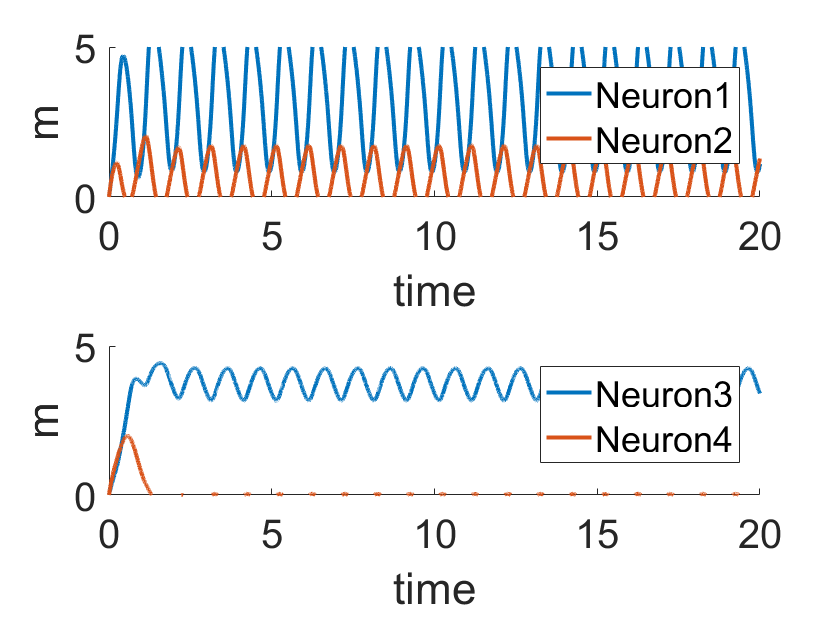
\includegraphics[width=0.5\textwidth]{fig/sat.png}
	\caption{A high positive coupling strengh on a neuronal oscillator excited by a periodic signal on the neuron 1.}\label{sat}
\end{figure}

\begin{figure}[!h]
	\centering
	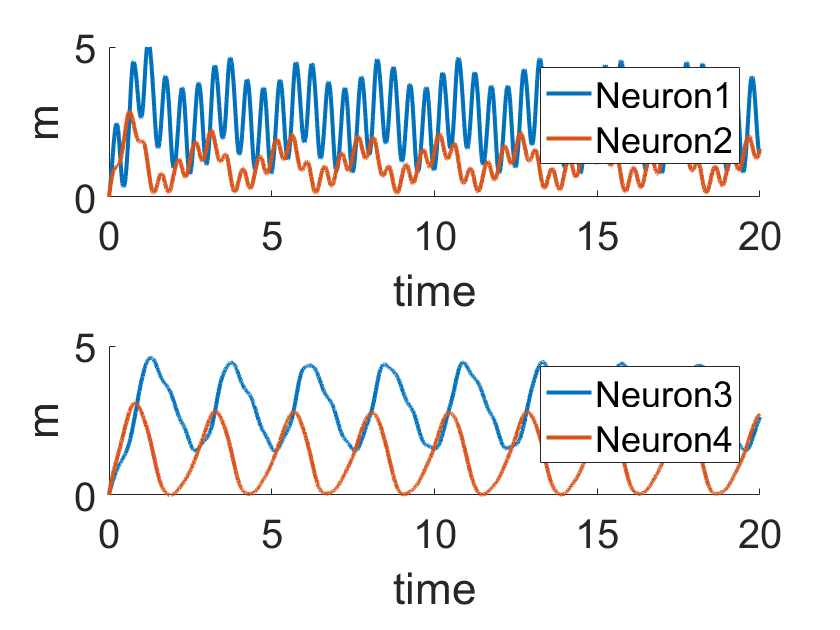
\includegraphics[width=0.5\textwidth]{fig/dd.png}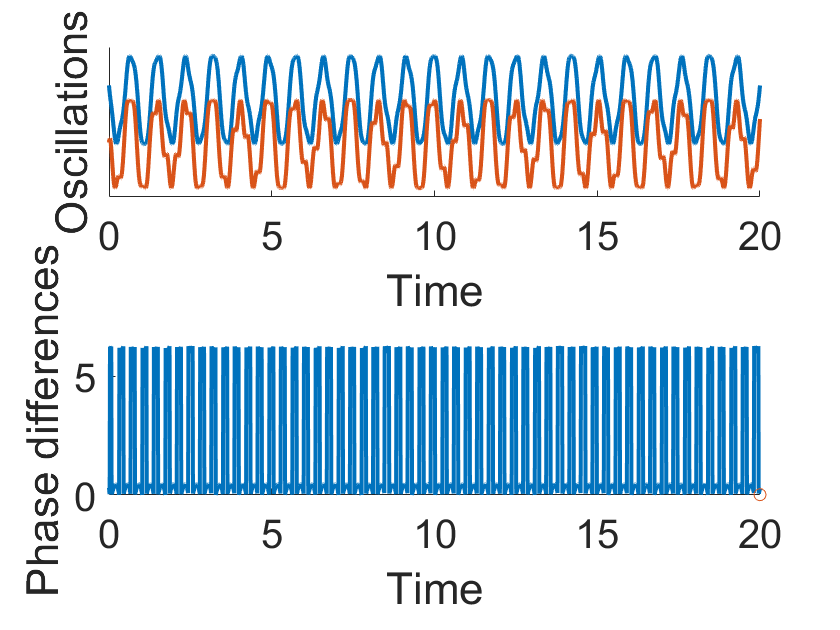
\includegraphics[width=0.5\textwidth]{fig/chao.png}
	\caption{On the left picture, a low constrain neuronal oscillator that doesnt saturate. On the right a chain phase oscillator with the same corresponding coupling strengh. In both case, a periodic input with a frequency 4 time higher than their intrinsic frequency is applied on one side.}\label{dd}
\end{figure}

Finally, one should remark that the oscillators don't always need to chose between the mechanical frequency and the intrinsic oscillation. Indeed for a well tuned system, the oscillator receiving sensory input can produce a superposition of intrinsic and mechanical oscillation. This normally happens if one of these frequencies is much higher than the other (see Figure \ref{dd}). Interestingly this is a behaviour that can also be observed for phase oscillators. Moreover, it is important to note that in both cases, the second oscillator is minimally affected by the high frequency oscillation.



\subsection{Arnold tongue (bonus)}

In order to find out more generally what combinations of values for the coupling strength and for the intrinsic frequencies of the oscillators lead to synchronization between the coupled neural oscillators, many different simulations were run using various values for parameters and tested for phase locking. For this, a definition of phase-locked oscillators was necessary. It was chosen to define to neural oscillators to in synchrony, if their resulting frequencies differed by less than a small value $\epsilon$. For our purpose, $\epsilon$ was set to 0.02, which allowed to test a range of parameter value couples for the model. The result of this round of simulations lead to a plot showing an approximation of the Arnold tongue for synchrony of two coupled neural oscillators with respect to the parameters (see Figure \ref{fig:bonus}). For this purpose the coupling strength was kept negative between 0 and -2, thus neglecting positive values of coupling since negative values had been shown to have better properties than positive ones for the coupling. The frequencies were not varied in all possible ranges; instead the time constant of one oscillator was kept constant at 0.04, while the time constant of the other oscillator was varied. However, the value plotted in figure \ref{fig:bonus} corresponds to the ratio between the time constants. Since the ratio was varied between 1 and 4, the time constant of the second oscillator was varied between 0.04 and 0.16. The resulting Arnold tongue shows that for time constant ratio close to one (meaning similar time constants for both oscillators), the system can synchronize even if the coupling strength is weak. Inversely, if the time constant ratio is big, the system only synchronizes, if the coupling strength is strong. Perhaps more surprisingly, it seems that around a time constant ratio of 3, a wall seems to be present beyond which none of the tested coupling strengths is sufficiently strong to bring the system into phase locking.

\begin{figure}[!h]
	\centering
	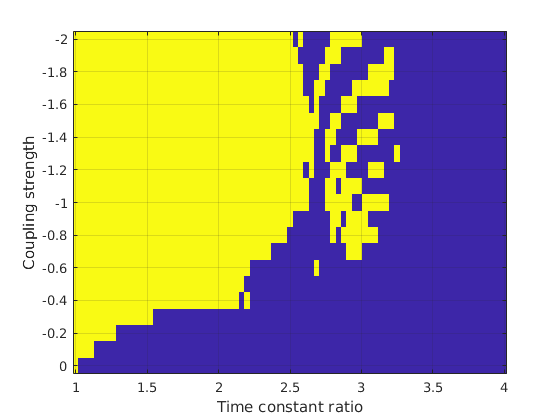
\includegraphics[width=0.5\textwidth]{fig/figurebonus_arnold.png}
	\caption{Experimental Arnold tongue, showing which pairs of values for coupling strength and time constant ratio of two coupled neural oscillators lead to synchrony between the oscillators. Yellow regions show parameter values that lead to synchrony and and blue regions show parameter values that didn't lead to synchrony.}
	\label{fig:bonus}
\end{figure}
	
\end{document}
